% %%%%%%%%%%%%%%%%%%%%%%%%%%%%%%%%%%%%%%%%%%%%%%%%%%%%%%%%%%%%%%%%%%%%%
% %% Background %%
% Hardware Challenges
% %%%%%%%%%%%%%%%%%%%%%%%%%%%%%%%%%%%%%%%%%%%%%%%%%%%%%%%%%%%%%%%%%%%%%

\section{Hardware Challenges for Sparse Matrix Computation}
\label{sec:bg:hwchallenges}

In the previous section we presented a brief background on matrix multiplication without considering the underlying hardware.
Although the various \emph{sparse formats} reduce the memory footprint, they have the disadvantage that indirect accesses are required, which creates data-dependencies and reduces the effectiveness of caches.
As we have seen, with all three algorithms, at least some of the accesses are non-sequential.
The lack of spatial locality for these accesses reduces the benefit of having caches.
In other words, a full cache line is loaded, but only a few entries are read or modified.
Moreover, the matrices of interest are extremely large and even the non-zero elements, and associated \emph{metadata}, can not generally fit in the cache.
Depending on the algorithm, successive accesses to the same element may be too far apart to benefit from temporal locality in the cache.
% TODO: find the reference

% Perhaps we can add a reference to Yves's background paper where it was stated
% that with typical sparse matrix formats ~50% of the data brought into the
% cache is unused.

%% INNER PRODUCT
In an \algo{IP} algorithm, the $A$-\emph{metadata} needs to be read to indirectly access the $B$-matrix (or $b$-vector), which may itself be stored in a \emph{sparse format}.
In this case, the algorithm needs to check if the non-zero $A$-indices are present in $B$ (or $b$). If an index appears in neither list, there is no need to perform the multiplication (\emph{ineffectual operation}).
More generally, this problem applies to \emph{fibers} and is called the \emph{intersection} search. As a minimum, this requires reading all the \emph{metadata} for $A$ and $B$ (or $b$), and identifying those present in both.

%%%% VL %%%%
In Algorithm~\ref{alg:bg:IPSpMSpMCSR}, we present the pseudo-code for an \emph{inner-product} SpMSpM with $A$ and $B$ stored in \emph{(UOP, CP) row-major} (\emph{CSR}) and \emph{column-major} (\emph{CSC}) formats, respectively.
The outer loop~(\emph{M}), iterates over the rows of $A$, and the first step is to identify the start (\emph{A\_current\_ptr}) and end column (\emph{A\_next\_ptr}) in the \emph{CSR} \emph{metadata}.
The middle-loop (\emph{n}) iterates over the columns of $B$.
The inner-loop iterates over the elements of the current row of $A$, and for each index (\emph{A\_pos}), a search is performed in the \emph{metadata} of $B$, to see if the corresponding index in $B$ is present.
Assuming it is ($B\_pos \neq -1$), the \emph{partial sum} is computed and then accumulated.
This example highlights the need to efficiently search for the intersection of indices in the \emph{metadata} of the inputs.

Different algorithms can be used to address the \emph{intersection} search, depending on whether the elements are sorted.
When the elements are sorted, the \emph{intersection} becomes a merge and generally requires $2 \times k-1$ comparisons (in some cases the number of comparisons can be reduced~\cite{Baeza-Yates2010_Intersection}).
As we will see in Section~\ref{cha:soa}, certain accelerators provide support for performing this intersection operation directly in hardware.

\begin{algorithm}
    \caption{\acrshort{ip} \acrshort{spmspm} Performing \Gls{intersection} Searches with \acrshort{csr} and \acrshort{csc} Formats}
    \label{alg:bg:IPSpMSpMCSR}
    %
    \KwData{$A(M, K)$ in \acrshort{csr}: $\mathit{A.val}, \mathit{A.idx}, \mathit{A.ptr}$}
    \KwData{$B(K, N)$ in \acrshort{csc}: $\mathit{B.val}, \mathit{B.idx}, \mathit{B.ptr}$}
    \KwData{$C(M, N)$ in \gls{dFormat} (for readability)}
    \KwResult{$C = A \times B$}
    \BlankLine
    \For(\tcp*[f]{Iterations over the rows of A}){$i \in \ldb 0, M-1 \rdb$}{
        \For(\tcp*[f]{Iterations over the columns of B}){$j \in \ldb 0, N-1 \rdb$}{
            $acc \gets 0$; $pos_B \gets \mathit{B.ptr}_j$\;
            \For{$pos_A \in \ldb \mathit{A.ptr}_i, \mathit{A.ptr}_{i+1}-1 \rdb$}{
                \tcp{Iterations over the non-zero elements of the i-th row of A}
                $k_A \gets \mathit{A.idx}_{pos_A}$\;
                \tcp{Column-index of the (i, $pos_A$) non-zero element of A}
                $(\mathit{isMatch}, pos_B) \gets \mathit{IntersectionSearch}(k_A, j, pos_B, \mathit{B.idx}, \mathit{B.ptr})$\;
                \tcp{Return true and the matching $pos_B$ if $idx$ exists in the j-th column of B}
                \If(\tcp*[f]{If indices did match}){$\mathit{isMatch}$}{
                    $acc \gets acc + \mathit{A.val}_{pos_A} \times \mathit{B.val}_{pos_B}$\;
                    \tcp{Local partial sum accumulation}
                }
            }
            $C_{i,j} \gets acc$\tcp*[r]{Write in memory of the resulting (i, j) element of C}
        }
    }
    \BlankLine
    \Fn{$\mathit{IntersectionSearch}(k_A, j, pos_B, \mathit{B.idx}, \mathit{B.ptr})$}{
        \tcp{Naive intersection search allowing the i-th row of A and the j-th column of B to be traversed only once at iteration (i, j)}
        \While{$\mathit{B.idx}_{pos_B} < k_A$ \textbf{and} $pos_B < \mathit{B.ptr}_{j+1}$}{
            $pos_B \gets pos_B + 1$\;
        }
        \If(\tcp*[f]{Returns true if indices from A and B match}){$\mathit{B.idx}_{pos_B} = k_A$}{
            \textbf{return} $(true, pos_B)$\;
        }
        \textbf{return} $(false, pos_B)$\;
    }
\end{algorithm}
%%%%%%%%%%%%

%% OUTER PRODUCT
In an \algo{OP} algorithm, the inputs are accessed sequentially, but the updates of the output require indirect accesses.
The pattern of the accesses, while the output is generated, is non-sequential and determined by the structure of the input.
Furthermore, if these \emph{random}\footnote{We use the term \emph{random} to mean accesses are irregular and difficult to predict.} updates provoke cache misses where only one word within a cache-line is modified, the bandwidth to external memory is poorly utilized.
The \algo{OP} algorithm generates several \emph{partial outputs} (\emph{POs}) that must be accumulated to obtain the final output.
We can identify two strategies: \emph{immediate update} and \emph{deferred update}.
In the former, the final output is immediately updated as each \emph{partial sum} is generated.
If the output is stored using a \emph{sparse format}, either the index being updated does not yet exist, and the new \emph{partial sum} must be inserted.
Or, if it exists, a lookup must be done to locate it, the update performed and the result written back.
The problem associated with combining the \emph{POs} is called \emph{reduction}.

%%%% VL %%%%
In Algorithm~\ref{alg:bg:OPSpMSpMCSR}, we present the pseudo-code for an \emph{outer-product} SpMSpM using \emph{immediate update} with A and $B$ stored in \emph{(UOP, CP) column-major} (\emph{CSC}) and \emph{row-major} (\emph{CSR}) formats, respectively.
The outer loop~(\emph{K}), iterates over the rows of A and the columns of $B$ (common rank), and the first step is to identify the start (\emph{A\_current\_ptr, B\_current\_ptr}) and end fibers (\emph{A\_next\_ptr},\emph{B\_next\_ptr}) in the \emph{metadata}.
The middle-loop (\emph{A\_pos}) iterates over the elements of the current column of A.
The inner-loop (\emph{B\_pos}) iterates over the elements of the current row of $B$.
Because we only iterate over the non-zero values, there is no need for a search.
The \emph{partial sum} is then computed. Finally, it must be accumulated to $C_{A\_ind,B\_ind}$.
These accesses are non-sequential, making it necessary to lookup the value in $C$, update it, and write it back, which is performed by the \emph{REDUCTION()} function in the pseudo-code.

% ref for merging methods to add?

\begin{algorithm}
    \caption{\acrshort{op} \acrshort{spmspm} Performing \Gls{reduction} with \acrshort{csr} and \acrshort{csc} Formats}
    \label{alg:bg:OPSpMSpMCSR}
    %
    \KwData{$A(M, K)$ in \acrshort{csr}: $\mathit{A.val}, \mathit{A.idx}, \mathit{A.ptr}$}
    \KwData{$B(K, N)$ in \acrshort{csc}: $\mathit{B.val}, \mathit{B.idx}, \mathit{B.ptr}$}
    \KwData{$\mathit{PO}_k(M, N)$ for all $k \in \ldb 0, K-1 \rdb$ in \acrshort{coo}: $\mathit{PO_k.val}, \mathit{PO_k.row}, \mathit{PO_k.col}$}
    \KwData{$C(M, N)$ in \gls{dFormat} (for readability)}
    \KwResult{$C = A \times B$}
    \BlankLine
    \tcp{* * * `Immediate updates' version * * *}
    \For(\tcp*[f]{Iterations over the columns of A and the rows of $B$}){$k \in \ldb 0, K-1 \rdb$}{
        \For{$pos_A \in \ldb \mathit{A.ptr}_k, \mathit{A.ptr}_{k+1} \rdb$}{
            \tcp{Iterations over the non-zero elements of the k-th column of A}
            $i_A \gets \mathit{A.idx}_{pos_A}$\tcp*[r]{Row-index of the ($pos_A$, k) non-zero element of A}
            \For{$pos_B \in \ldb \mathit{B.ptr}_k, \mathit{B.ptr}_{k+1} \rdb$}{
                \tcp{Iterations over the non-zero elements of the k-th row of B}
                $j_B \gets \mathit{B.idx}_{pos_B}$\;
                \tcp{Column-index of the (k, $pos_B$) non-zero element of B}
                $C_{i_A, j_B} \gets C_{i_A, j_B} + \mathit{A.val}_{pos_A} \times \mathit{B.val}_{pos_B}$\;
                \tcp{Reduction (to memory) of the partial sum into the ($i_A$, $j_B$) element of C (immediate update)}
            }
        }
    }
    \BlankLine
    \tcp{* * * `Deffered updates' version * * *}
    \tcp{Multiply phase}
    \For(\tcp*[f]{Iterations over the columns of A and the rows of $B$}){$k \in \ldb 0, K-1 \rdb$}{
        $pos_\mathit{PO} \gets 0$\;
        \For{$pos_A \in \ldb \mathit{A.ptr}_k, \mathit{A.ptr}_{k+1} \rdb$}{
            \tcp{Iterations over the non-zero elements of the k-th column of A}
            $i_A \gets \mathit{A.idx}_{pos_A}$\tcp*[r]{Row-index of the ($pos_A$, k) non-zero element of A}
            \For{$pos_B \in \ldb \mathit{B.ptr}_k, \mathit{B.ptr}_{k+1} \rdb$}{
                \tcp{Iterations over the non-zero elements of the k-th row of B}
                $j_B \gets \mathit{B.idx}_{pos_B}$\;
                \tcp{Column-index of the (k, $pos_B$) non-zero element of B}
                $\mathit{PO_k.row}_{pos_\mathit{PO}} \gets i_A$\;
                $\mathit{PO_k.col}_{pos_\mathit{PO}} \gets j_B$\;
                $\mathit{PO_k.val}_{pos_\mathit{PO}} \gets \mathit{A.val}_{pos_A} \times \mathit{B.val}_{pos_B}$\; 
                \tcp{The k-th partial sum of the ($i_A$, $j_B$) element of C is stored in memory in the k-th partial output}
                $pos_\mathit{PO} \gets pos_\mathit{PO} + 1$\;
            }
        }
        \tcp{Each partial output is generated sorted, row-wise}
    }
    \tcp{Merge phase}
    \For(\tcp*[f]{Naive serial merge of the K partial outputs}){$k \in \ldb 0, K-2 \rdb$}{
        % $\mathit{MergedPO} \gets \{\}$\;
        % $pos_1 \gets 0$; $pos_2 \gets 0$; $pos_M \gets 0$\;
        % \While{$pos_1 < length(\mathit{PO}_k)$ \textbf{and} $pos_2 < length(\mathit{PO}_{k+1})$}{
        %     \If{$\mathit{PO_k.row}_{pos_1} < \mathit{PO_{k+1}.row}_{pos_2}$}{
        %         $\mathit{MergedPO}_{pos_M} \gets \mathit{PO_k}_{pos_1}$\;
        %         $pos_1 \gets pos_1 + 1$\;
        %     }
        %     \ElseIf{$\mathit{PO_k.row}_{pos_1} > \mathit{PO_{k+1}.row}_{pos_2}$}{
        %         $\mathit{MergedPO}_{pos_M} \gets \mathit{PO_{k+1}}_{pos_2}$\;
        %         $pos_2 \gets pos_2 + 1$\;
        %     }
        %     \Else{
        %         \If{$\mathit{PO_k.col}_{pos_1} < \mathit{PO_{k+1}.col}_{pos_2}$}{
        %             $\mathit{MergedPO}_{pos_M} \gets \mathit{PO_k}_{pos_1}$\;
        %             $pos_1 \gets pos_1 + 1$\;
        %         }
        %         \ElseIf{$\mathit{PO_k.col}_{pos_1} > \mathit{PO_{k+1}.col}_{pos_2}$}{
        %             $\mathit{MergedPO}_{pos_M} \gets \mathit{PO_{k+1}}_{pos_2}$\;
        %             $pos_2 \gets pos_2 + 1$\;
        %         }
        %         \Else{
        %             $\mathit{MergedPO}_{pos_M} \gets \mathit{PO_k}_{pos_1} + \mathit{PO_{k+1}}_{pos_2}$\;
        %             $pos_1 \gets pos_1 + 1$\;
        %             $pos_2 \gets pos_2 + 1$\;
        %         }
        %     }
        %     $pos_M \gets pos_M + 1$\;
        % }
        % \While{$pos_1 < length(\mathit{PO}_k)$}{
        %     $\mathit{MergedPO}_{pos_M} \gets \mathit{PO_k}_{pos_1}$\;
        %     $pos_1 \gets pos_1 + 1$; $pos_M \gets pos_M + 1$\;
        % }
        % \While{$pos_2 < length(\mathit{PO}_{k+1})$}{
        %     $\mathit{MergedPO}_{pos_M} \gets \mathit{PO_{k+1}}_{pos_2}$\;
        %     $pos_2 \gets pos_2 + 1$; $pos_M \gets pos_M + 1$\;
        % }
        $\mathit{PO}_{k+1} \gets \mathit{2DListsMerge}(\mathit{PO}_k, \mathit{PO}_{k+1})$\;
        % $\mathit{PO}_{k+1} \gets \mathit{MergedPO}$\;
    }
    \tcp{$\mathit{PO}_{K-1}$ is C stored in COO format}
    \For{$pos \in \ldb 0, length(\mathit{PO}_{K-1})-1 \rdb$}{
        \tcp{Update C (dense) from the fully merged partial outputs}
        $i \gets \mathit{PO_{K-1}.row}_{pos}$\;
        $j \gets \mathit{PO_{K-1}.col}_{pos}$\;
        $C_{i, j} \gets \mathit{PO_{K-1}.val}_{pos}$\tcp*[r]{Write in memory of the (i, j) element of C}
    }
\end{algorithm}
%%%%%%%%%%%%

% This paragraph covers deferred updates
To avoid the complexities of the indirect accesses with \emph{immediate updates}, the \emph{partial sums} can be stored and the accumulation can be deferred. One such technique is called \emph{output batching}~\cite{Kiriansky2016_Milk}. With this technique, tuples containing the index and the \emph{partial sum} are streamed sequentially to memory. Then, during a second pass, they are read back and the accumulations are performed, an approach which results in sequential memory accesses during the first pass, with the downside that the volume of data transferred to memory is increased.
%%%% VL %%%%
The different strategies for dealing with these updates are shown in Figure~\ref{fig:bg:OutputUpdatesStategies}.
%%%%%%%%%%%%
As we will see, hardware accelerators may combine the \emph{immediate} and \emph{deferred update} techniques to optimize memory bandwidth.
%%%% VL %%%%
\begin{figure}
    \begin{minipage}[b]{0.69\linewidth}
        \begin{figure}[H]% Does it go with a taxonomy in the comparison section?
            \centering
            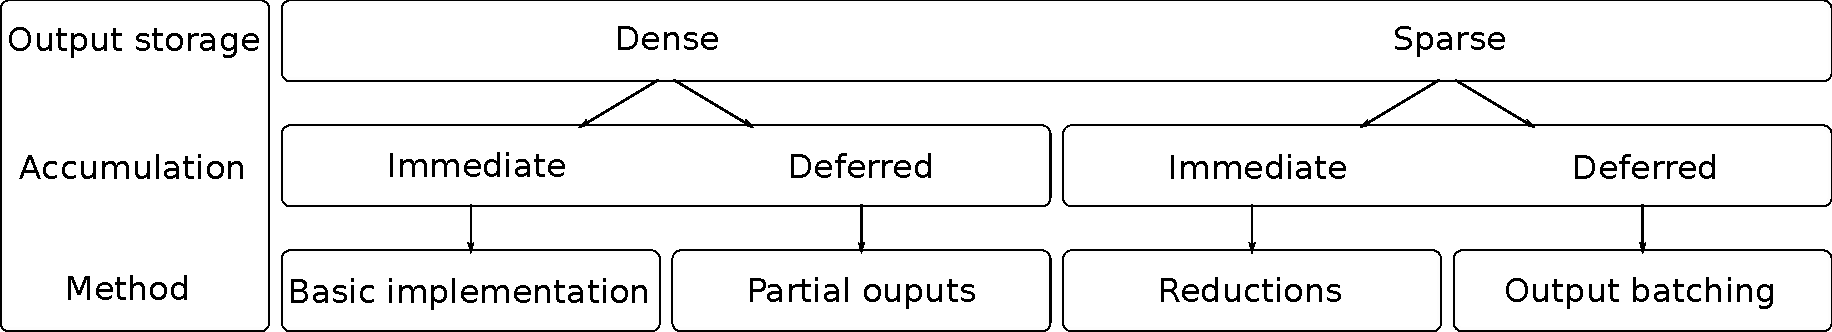
\includegraphics[width=\textwidth]{Chapter_Background/Figures/PDF/OutputUpdates.pdf}
            \caption{Strategies for Dealing with Random Output Updates in Outer Product Algorithms}
            \label{fig:bg:OutputUpdatesStategies}
        \end{figure}
    \end{minipage}
    \hfill
    \begin{minipage}[b]{0.29\linewidth}
        \begin{figure}[H]
            \centering
            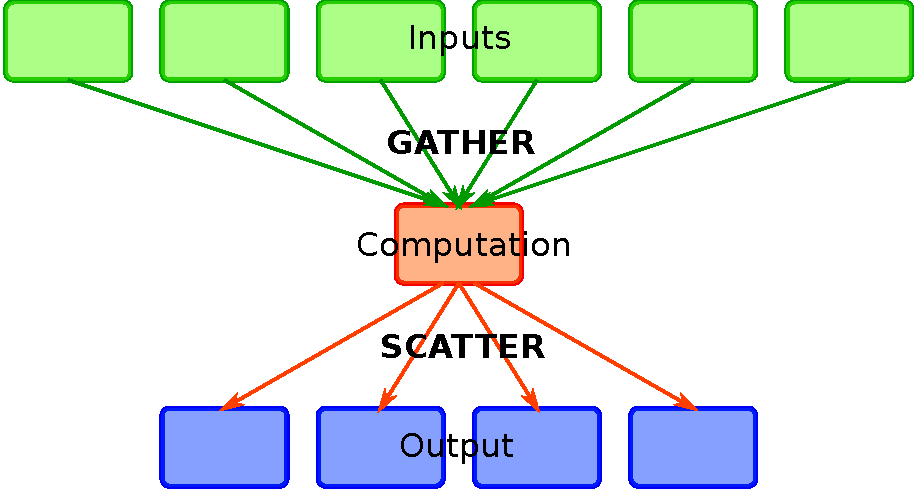
\includegraphics[width=\textwidth]{Chapter_Background/Figures/PDF/GatherScatter.pdf}
            \caption{\emph{Gather} and \emph{Scatter} Illustration}
            \label{fig:bg:gatherscatter}
        \end{figure}
    \end{minipage}
\end{figure}
%%%%%%%%%%%%
In Table~\ref{tab:bg:AlgosHWComp}, we summarize the previously discussed advantages and hardware challenges for each algorithm, including \algo{Gust} which presents a trade-off between \algo{IP} and \algo{OP}.

\begin{table}
    \centering
    \caption{Comparison of Advantages and Challenges with Matrix Multiplication Algorithms}
    \label{tab:bg:AlgosHWComp}
    \begin{tblr}{
            width = {\linewidth},
            colspec = {X[-1,c] X[-1,c] *{3}{X[j]}}, % rowspec
            rows = {m, font=\scriptsize},
            colsep = {4pt},
            row{1-Z} = {rowsep=1pt, black!2},
            row{1} = {c, font=\bfseries\scriptsize, black!5},
            column{1-2} = {font=\bfseries\scriptsize},
            cell{2}{1} = {r=2}{c},
            cell{4-Z}{1} = {c=2}{c},
            cell{5}{3} = {c=2}{l},
            cell{2}{Z} = {c},
            % hlines, vlines,
            % rulesep = {-1pt},
            hline{1,Z} = {2pt}, % Z for last
            hline{2} = {1pt},
            hline{3} = {2-Z}{0.5pt},
            hline{4-Y} = {0.5pt},
            vline{3} = {2-Z}{0.5pt},
        }
        &
        &
        \acrfull{ip} &
        \acrfull{op} &
        \acrfull{gust} \\
        %
        {Access \\ Count} &
        \acrshort{mv} &
        \textbf{\textit{A}:} once ; \textbf{\textit{b}:} $nnz(A)$ ; \textbf{\textit{c}:} once &
        \textbf{\textit{A}:} once ; \textbf{\textit{b}:} once ; \textbf{\textit{c}:} $nnz_{r}(A)$ &
        \emph{N/A} \\
        %
        &
        \acrshort{mm} &
        \textbf{\textit{A}:} $N$ ; \textbf{\textit{B}:} $nnz_{r}(A).M$ ; \newline \textbf{\textit{C}:} once &
        \textbf{\textit{A}:} once ; \textbf{\textit{B}:} $nnz_{c}(A)$ \newline \textbf{\textit{C}:} $\sim nnz_{r}(A).nnz_{c}(B)/K$ &
        \textbf{\textit{A}:} once ; \textbf{\textit{B}:} $nnz_{c}(A)$ \newline \textbf{\textit{C}:} $\sim nnz_{r}(A).nnz_{c}(B)/K$ \\
        %
        {Sequential \\ Accesses} &
        &
        Accesses to $A$ and $C$ &
        Accesses to $A$ and $B$ &
        Accesses to $A$ and $C$ \newline Accesses to $B$-rows \\
        %
        {Input \\ Format} &
        &
        {Accesses to $A$ and $B$ benefit from alternate formats (\emph{CSR} and \\ \emph{CSC})}&
        &
        Allows consistent format for $A$ and $B$ \\
        %
        {Parallelism \\ Opportunity} &
        &
        Possible with \gls{tiling} &
        Generation of \emph{POs} over \emph{common rank} of $A$ and $B$ &
        Reading $A$-rows and updating $C$-rows \\
        %
        {Reuse \\ Opportunity} &
        &
        Potentially $B$, but limited by its size &
        An $A$-column or $B$-row while computing \emph{POs} &
        $A$ set of $B$-rows, based on non-zero elements of $A$-rows \\ %Based on non-zero elements of $A$-rows, a set of $B$-rows are reused
        %
        Challenges &
        &
        \emph{Intersection} search between non-zero elements in $A$ and $B$ &
        Storage for \emph{POs} or in-place  \emph{merge} and \emph{reduce} &
        \emph{Merge} and \emph{reduce} of  \emph{PO rows} \\
    \end{tblr}
\end{table}

% \begin{table}
%     \newlength{\fstC}
%     \setlength{\fstC}{1.00cm}
%     \newlength{\scdC}
%     \setlength{\scdC}{0.65cm}
%     \newlength{\fstAndScdC}
%     \setlength{\fstAndScdC}{2.00cm}
%     \newlength{\lstC}
%     \setlength{\lstC}{4.03cm}
%     \centering
%     \caption{Comparison of Advantages and Challenges with Matrix Multiplication Algorithms}
%     \label{tab:bg:AlgosHWComp}
%     % \footnotesize
%     \scriptsize
%     \begin{tabular}{|>{\arraybackslash\centering}m{\fstC} >{\arraybackslash\centering}m{\scdC}|| *{3}{>{\arraybackslash}m{\lstC}|}}
%         \hhline{--||---}
%         &
%         &
%         \multicolumn{1}{c|}{\textbf{\acrfull{ip}}} &
%         \multicolumn{1}{c|}{\textbf{\acrfull{op}}} &
%         \multicolumn{1}{c|}{\textbf{\acrfull{gust}}} \\
%         %
%         \hhline{==::===}
%         \multirow{3}{\fstC}{\centering\textbf{Access Count}} &
%         \multicolumn{1}{|>{\arraybackslash\centering}m{\scdC}||}{\textbf{MV}} &
%         \textbf{\textit{A}:} once ; \textbf{\textit{b}:} $nnz(A)$ ; \textbf{\textit{c}:} once &
%         \textbf{\textit{A}:} once ; \textbf{\textit{b}:} once ; \textbf{\textit{c}:} $nnz_{r}(A)$ &
%         \multicolumn{1}{c|}{\emph{N/A}} \\
%         %
%         \hhline{~-||---}
%         &
%         \multicolumn{1}{|>{\arraybackslash\centering}m{\scdC}||}{\textbf{MM}} &
%         \textbf{\textit{A}:} $N$ ; \textbf{\textit{B}:} $nnz_{r}(A).M$ ; \newline \textbf{\textit{C}:} once &
%         \textbf{\textit{A}:} once ; \textbf{\textit{B}:} $nnz_{c}(A)$ \newline \textbf{\textit{C}:} $\sim nnz_{r}(A).nnz_{c}(B)/K$ &
%         \textbf{\textit{A}:} once ; \textbf{\textit{B}:} $nnz_{c}(A)$ \newline \textbf{\textit{C}:} $\sim nnz_{r}(A).nnz_{c}(B)/K$ \\
%         %
%         \hhline{--||---}
%         \multicolumn{2}{|>{\arraybackslash\centering}m{\fstAndScdC}||}{\textbf{Sequential Accesses}} &
%         Accesses to $A$ and $C$ &
%         Accesses to $A$ and $B$ &
%         Accesses to $A$ and $C$ \newline Accesses to $B$-rows \\
%         %
%         \hhline{--||---}
%         \multicolumn{2}{|>{\arraybackslash\centering}m{\fstAndScdC}||}{\textbf{Input Format}} &
%         \multicolumn{2}{l|}{\begin{minipage}{7.00cm} Accesses to $A$ and $B$ benefit from alternate formats (\emph{CSR} and \emph{CSC}) \end{minipage}} & 
%         Allows consistent format for $A$ and $B$ \\
%         %
%         \hhline{--||---}
%         \multicolumn{2}{|>{\arraybackslash\centering}m{\fstAndScdC}||}{\textbf{Parallelism Opportunity}} &
%         Possible with \gls{tiling} &
%         Generation of \emph{POs} over \emph{common rank} of $A$ and $B$ &
%         Reading $A$-rows and updating $C$-rows \\
%         %
%         \hhline{--||---}
%         \multicolumn{2}{|>{\arraybackslash\centering}m{\fstAndScdC}||}{\textbf{Reuse Opportunity}} &
%         Potentially $B$, but limited by its size &
%         An $A$-column or $B$-row while computing \emph{POs} &
%         $A$ set of $B$-rows, based on non-zero elements of $A$-rows \\ %Based on non-zero elements of $A$-rows, a set of $B$-rows are reused
%         %
%         \hhline{--||---}
%         \multicolumn{2}{|>{\arraybackslash\centering}m{\fstAndScdC}||}{\textbf{Challenges}} &
%         \emph{Intersection} search between non-zero elements in $A$ and $B$ &
%         Storage for \emph{POs} or in-place  \emph{merge} and \emph{reduce} &
%         \emph{Merge} and \emph{reduce} of  \emph{PO rows} \\
%         %
%         \hhline{--||---}
%     \end{tabular}
% \end{table}

%%%% VC %%%%
The issues presented with \algo{IP} and \algo{OP} can be generalized to two concepts: \emph{gather} and \emph{scatter}.
%%%% VL %%%%
% The issues presented with \emph{inner-product} and \emph{outer-product} can be generalized to two concepts: \emph{gather} and \emph{scatter} (see Figure~\ref{fig:gatherscatter}).
%%%%%%%%%%%%
The \emph{gather} problem exists when the inputs are indirectly accessed, and need to be read from memory using \emph{metadata} to present the processor with the correct terms for computing the \emph{partial sums}. Typically, with \algo{IP}, the \emph{gather} problem is more difficult.
The \emph{scatter} problem exists when the order in which the output matrix/vector is generated is not sequential and is typically associated with the \algo{OP} algorithm.
In the case of \emph{tiling}, a hardware accelerator must handle both \emph{gather} and \emph{scatter}, creating a need for hardware support for both \emph{intersection} searches and \emph{reductions}.

\subsection{SpMSpM Algorithm Analysis}
\label{sec:bg:AnalyticalModel}

To better understand how the algorithms impact the number and types of memory accesses, we developed, and presented in Figure~\ref{fig:bg:AnalyticalModel_SpMSpM}, a model based on memory accesses counts. We identify five memory access patterns: (1) those where a matrix is read only once, thus there is no opportunity for reuse, (2) where the accesses are sequential, but a line is read multiple times, (3) where lines are read consecutively, but the accesses within a line are \emph{random}, (4) where the lines are accessed \emph{randomly}, but within a line the accesses are sequential, and (5) where the matrix elements are accessed multiple times, and with a \emph{random} access pattern.

For each of the three algorithms, we counted the number of read and write accesses, based on the density of the input matrices. We plotted the number of memory accesses in logarithmic scale for SpMSpM, based on a square matrix with $M = 10,000$. Indeed, the number of non-zero elements in $C$ depends on the structure of the input matrices and in this model, we have assumed the non-zero entries in the input matrices are uniformly, randomly distributed. This corresponds to a \emph{worst case} for sparse matrices (no spatial and temporal locality). Banded input matrices would, for example, have fewer non-zero elements in $C$.
In each graph, we have separated the accesses into $A$ (bottom), $B$ (middle) and $C$ (top). The colour code shows the access pattern, based on the five categories described above.

In the top-row of Figure~\ref{fig:bg:AnalyticalModel_SpMSpM} (graphs~\ding{192}, \ding{193} and~\ding{194}), we start by considering a naïve accelerator which has no local storage, thus all data comes from main memory. From these figures, we clearly see that \algo{IP} requires more accesses, as the $A$-matrix must be read N times (graph~\ding{192}). Whereas for \algo{OP} and \algo{Gust}, the $A$-matrix is read only once (thus the grey colour). For \algo{OP} and \algo{Gust} the total number of accesses is the same, however, with \algo{OP} (graph~\ding{193}), the accesses to $C$ are \emph{random} (red). With \algo{Gust} (graph~\ding{194}), the accesses to $B$ are sequential within the rows (orange) and the $C$-rows are generated sequentially (yellow), thus \algo{Gust} avoids having any fully \emph{random} accesses (red).

\begin{figure}
    \centering
    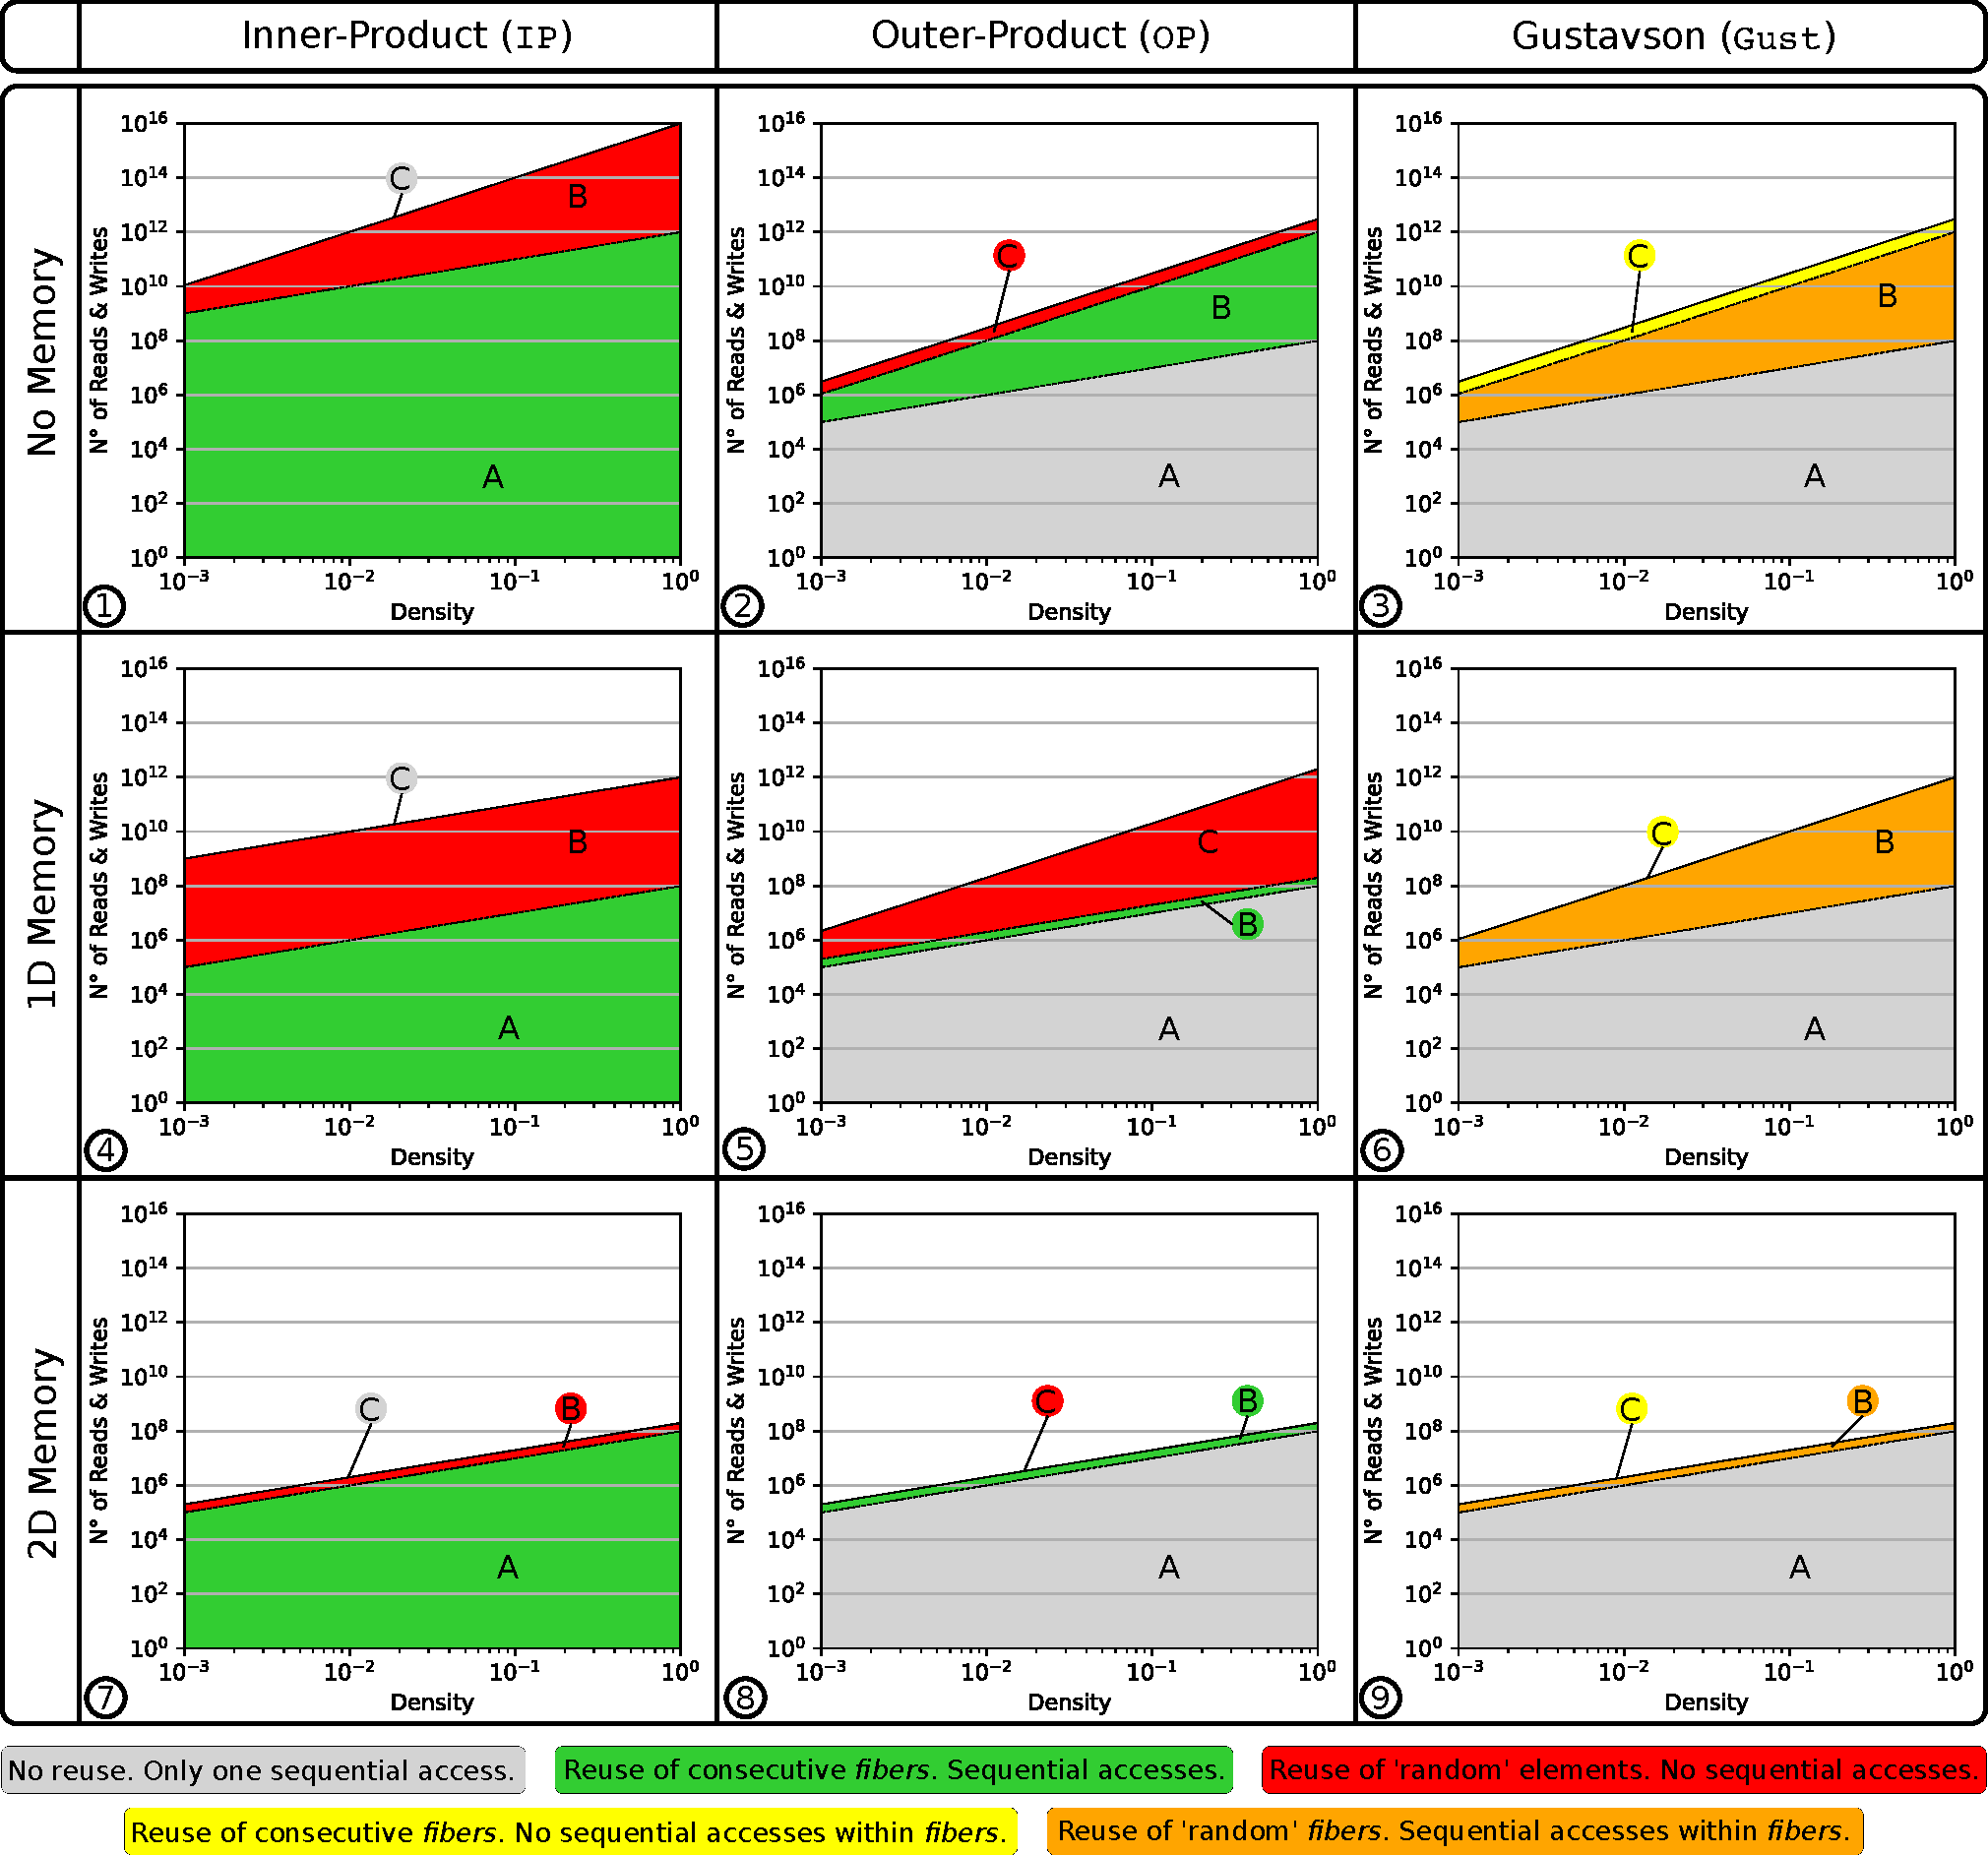
\includegraphics[width=\textwidth]{Chapter_Background/Figures/PDF/AnalyticalModel_SpMSpM.pdf}
    \caption{Model of Memory Access Counts Depending on Algorithm and Local Memory Size}
    \label{fig:bg:AnalyticalModel_SpMSpM}
\end{figure}

Since main memory accesses are the principal bottleneck, accelerators integrate local storage (such as buffers or caches). Thus, we consider the case of an accelerator with sufficient local memory to store one full row, per matrix. We assume this local storage is perfect (no misses) and re-calculate the number of remaining main memory accesses, as shown in the middle-row of Figure~\ref{fig:bg:AnalyticalModel_SpMSpM} (graphs~\ding{195}, \ding{196} and~\ding{197}). The matrices are assumed to be initially stored in main memory, thus they must be accessed at least once.
As can be seen, for \algo{IP} (graph~\ding{195}), the number of $A$-accesses is reduced, because rows are reused, thus the total number of $A$-accesses becomes equal to that in \algo{OP} and \algo{Gust}. For \algo{OP} (graph~\ding{196}), the single row buffer greatly reduces the number of $B$-accesses, however, it does nothing for $C$ (despite the appearance, due to the logarithmic scale). For \algo{Gust} (graph~\ding{197}), the single row buffer is sufficient to cache the \emph{reduction} operations in $C$, and thus, it now has fewer overall accesses than \algo{OP}. It is also interesting to note that \algo{OP} and \algo{Gust} scale better than \algo{IP} with lower densities, as seen by the shallower slope.

Finally, we have considered the extreme case where an accelerator has a buffer of sufficient size to store two matrices, which is shown in the bottom-row of Figure~\ref{fig:bg:AnalyticalModel_SpMSpM} (graphs~\ding{198}, \ding{199} and~\ding{200}). Although this case is not practical for large matrices, through the proper use of \emph{tiling} to locally reduce the dimensions of a sub-matrix, this case can be achieved at the level of a \emph{tile}. In this case, the total number of external accesses is equal for the three algorithms, as each matrix is accessed only once from main memory. For \algo{IP} (graph~\ding{198}), it is interesting to note that such a large buffer is needed to locally address the \emph{intersection} search in $B$. Similarly for \algo{OP} (graph~\ding{199}), a large storage is required to address the \emph{reductions} in $C$. For \algo{Gust}, in fact, it is not necessary to buffer the entire $B$-matrix. Indeed, buffering a few rows (corresponding to $nnz_{r}(A)$) is sufficient to achieve the number of accesses shown in graph~\ding{200}. This corresponds to an intermediate design point (multiple row buffers for $B$) not explicitly shown in the figure (between graphs~\ding{197} and~\ding{200}).

When viewed overall, Figure~\ref{fig:bg:AnalyticalModel_SpMSpM} highlights the benefits of \algo{Gust}. We clearly see that \algo{Gust} does not require any fully \emph{random} accesses (red). With a single row buffer, it is possible to address the \emph{reductions} in $C$. And, with a limited number of row buffers, the number of external memory accesses for $B$ can be reduced. Based on this analysis, it is clear that \algo{Gust} is the best algorithm for hardware implementation of SpMSpM.

% \begin{table}
%     \centering
%     \caption{Caption}
%     \label{tab:my_label}
%     \begin{tabular}{|c|| *{3}{>{\arraybackslash}m{4.15cm}|}}
%         \hhline{-||---}
%          & \textbf{Inner-Product (\algo{IP})} & \textbf{Outer-Product (\algo{OP})} & \textbf{Gustavson (\algo{Gust})} \\
%          \hhline{=::===}
%         \textbf{A$(M,K)$} & 0D: $nnz(A) \times N$ \newline 1D: $nnz(A)$ & 0D: $nnz(A)$ & 0D: $nnz(A)$ \\
%         \hhline{-||---}
%         \textbf{B$(K,N)$} & 0D: $nnz_{r}(A) \times nnz(B) \times M$ \newline $= nnz(A) \times nnz(B)$ \newline 1D: $nnz($B$) \times M$ \newline 2D: $nnz($B$)$ & 0D: $nnz_{c}(A) \times nnz_{r}($B$) \times K$ \newline $= nnz_{c}(A) \times nnz($B$)$ \newline 1D: $nnz_{r}($B$) \times K = nnz($B$)$ & 0D: $nnz_{r}(A) \times nnz_{r}($B$) \times M$ \newline $= nnz(A) \times nnz_{r}($B$)$ \newline 2D: $nnz($B$)$ \\
%         \hhline{-||---}
%         \textbf{C$(M,N)$} & 0D: $nnz(C) \times 2$ \newline (max: $M \times N \times 2$) & 0D: $nnz_{c}(A) \times nnz_{r}($B$) \times K \times 2$ \newline $= nnz_{c}(A) \times nnz($B$) \times 2$ \newline 2D: $nnz(C) \times 2$ \newline (max: $M \times N \times 2$) & 0D: $nnz_{r}(A) \times nnz_{r}($B$) \times M \times 2$ \newline $= nnz(A) \times nnz_{r}($B$) \times 2$ \newline 1D: $nnz(C) \times 2$ \newline (max: $M \times N \times 2$) \\
%         \hhline{-||---}
%     \end{tabular}
% \end{table}